% !TeX spellcheck = cs_CZ
{\tikzset{external/prefix={tikz/FYZII/}}
 \tikzset{external/figure name/.add={ch29_}{}}
%---------------------------------------------------------------------------------------------------
% file fey2ch29.tex
%---------------------------------------------------------------------------------------------------
%=========================== Kapitola Pohyb nábojů v elektrickém a magnetickém poli ================
\chapter{Pohyb nábojů v elektrickém a magnetickém poli}\label{fyz:IIchapXXIX}
\minitoc
  \section{Pohyb v homogenní elektrickém nebo magnetickém poli}\label{fyz:IIchapXXIXsecI}
  \section{Analyzátor hybnosti}\label{fyz:IIchapXXIXsecII}
  \section{Elektrostatická čočka}\label{fyz:IIchapXXIXsecIII}
  \section{Magnetická čočka}\label{fyz:IIchapXXIXsecIV}
  \section{Elektronový mikroskop}\label{fyz:IIchapXXIXsecV}
  \section{Stabilizující pole urychlovačů}\label{fyz:IIchapXXIXsecVI}
  \section{Fokusace pomocí střídavého gradientu}\label{fyz:IIchapXXIXsecVII}
  \section{Pohyb ve skřížených elektrických a magnetických polích}\label{fyz:IIchapXXIXsecVIII}
  \section{Příklady a cvičení}\label{fyz:IIchapXXIXsecIX}


    \begin{figure}[ht!] %\ref{fyz_fig623}
      \centering
      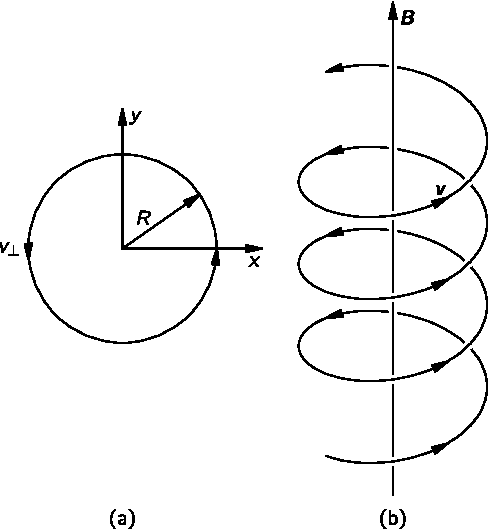
\includegraphics[width=0.7\linewidth]{fyz_fig623.pdf}
      \caption{
               (\cite[s.~707]{Feynman02})}
      \label{fyz_fig623}
    \end{figure}

    \begin{figure}[ht!]
      \centering
      \begin{tabular}{c}
        \subfloat[ ]{\label{fyz_fig624a}
          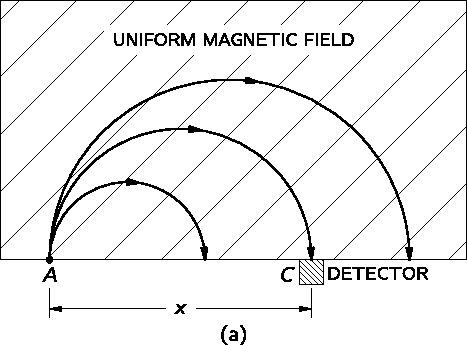
\includegraphics[width=0.3\linewidth]{fyz_fig624a.pdf}}               \\
        \subfloat[ ]{\label{fyz_fig624b}
          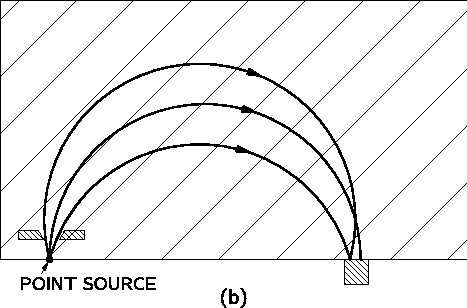
\includegraphics[width=0.3\linewidth]{fyz_fig624b.pdf}}
      \end{tabular}
      \label{fyz_fig624}
      \caption{
               (\cite[s.~748]{Feynman02})}
    \end{figure}

    \begin{figure}[ht!] %\ref{fyz_fig625}
      \centering
      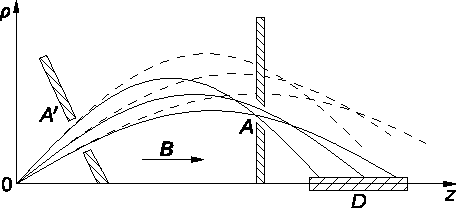
\includegraphics[width=0.7\linewidth]{fyz_fig625.pdf}
      \caption{
               (\cite[s.~707]{Feynman02})}
      \label{fyz_fig625}
    \end{figure}

    \begin{figure}[ht!] %\ref{fyz_fig626}
      \centering
      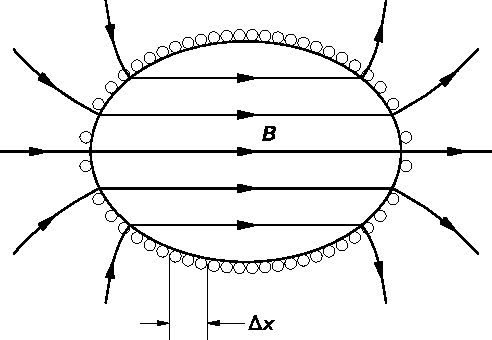
\includegraphics[width=0.7\linewidth]{fyz_fig626.pdf}
      \caption{
               (\cite[s.~707]{Feynman02})}
      \label{fyz_fig626}
    \end{figure}

    \begin{figure}[ht!] %\ref{fyz_fig627}
      \centering
      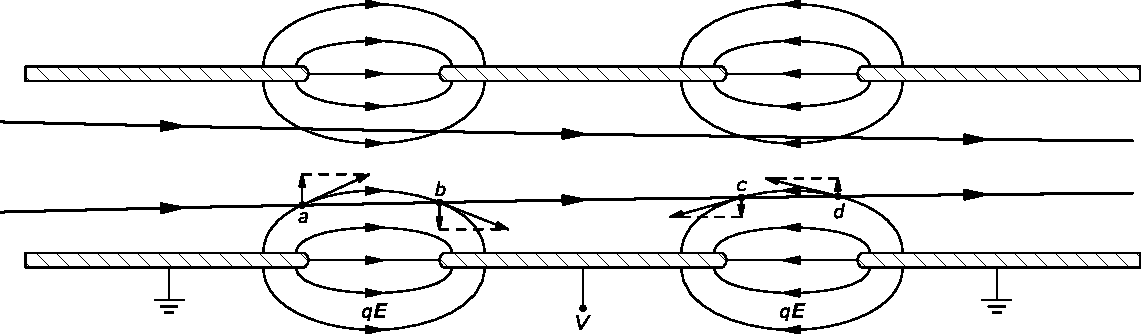
\includegraphics[width=0.7\linewidth]{fyz_fig627.pdf}
      \caption{
               (\cite[s.~707]{Feynman02})}
      \label{fyz_fig627}
    \end{figure}

    \begin{figure}[ht!] %\ref{fyz_fig628}
      \centering
      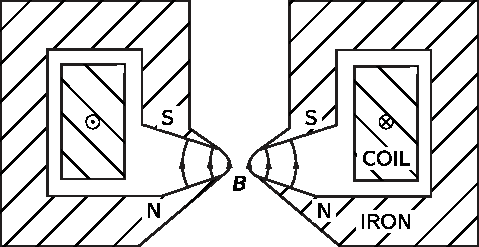
\includegraphics[width=0.7\linewidth]{fyz_fig628.pdf}
      \caption{
               (\cite[s.~707]{Feynman02})}
      \label{fyz_fig628}
    \end{figure}

    \begin{figure}[ht!] %\ref{fyz_fig629}
      \centering
      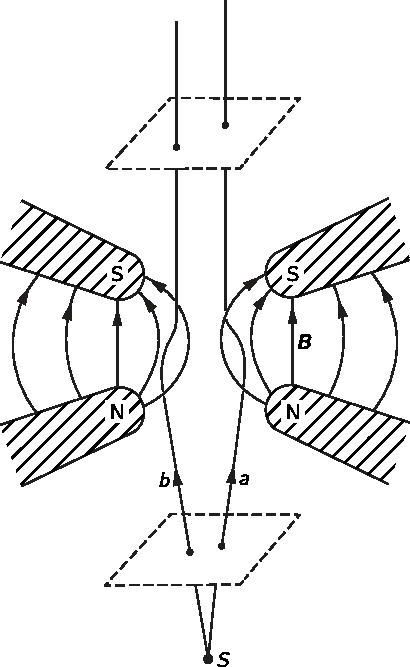
\includegraphics[width=0.7\linewidth]{fyz_fig629.pdf}
      \caption{
               (\cite[s.~707]{Feynman02})}
      \label{fyz_fig629}
    \end{figure}

    \begin{figure}[ht!] %\ref{fyz_fig630}
      \centering
      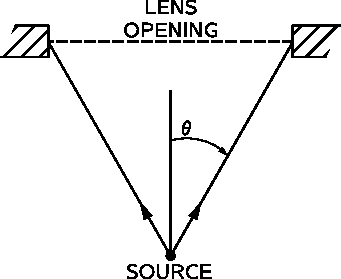
\includegraphics[width=0.7\linewidth]{fyz_fig630.pdf}
      \caption{
               (\cite[s.~707]{Feynman02})}
      \label{fyz_fig630}
    \end{figure}

    \begin{figure}[ht!] %\ref{fyz_fig631}
      \centering
      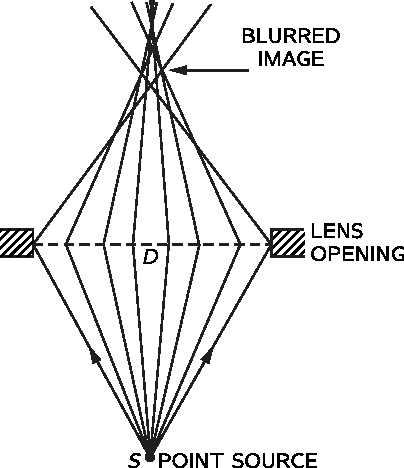
\includegraphics[width=0.7\linewidth]{fyz_fig631.pdf}
      \caption{
               (\cite[s.~707]{Feynman02})}
      \label{fyz_fig631}
    \end{figure}

    \begin{figure}[ht!] %\ref{fyz_fig632}
      \centering
      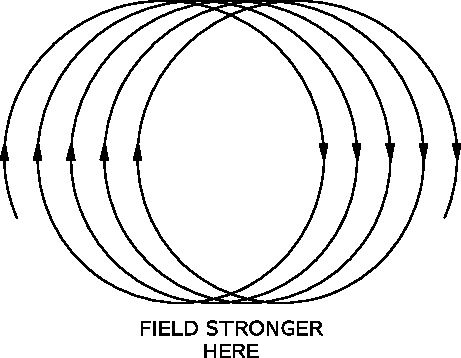
\includegraphics[width=0.7\linewidth]{fyz_fig632.pdf}
      \caption{
               (\cite[s.~707]{Feynman02})}
      \label{fyz_fig632}
    \end{figure}

    \begin{figure}[ht!] %\ref{fyz_fig633}
      \centering
      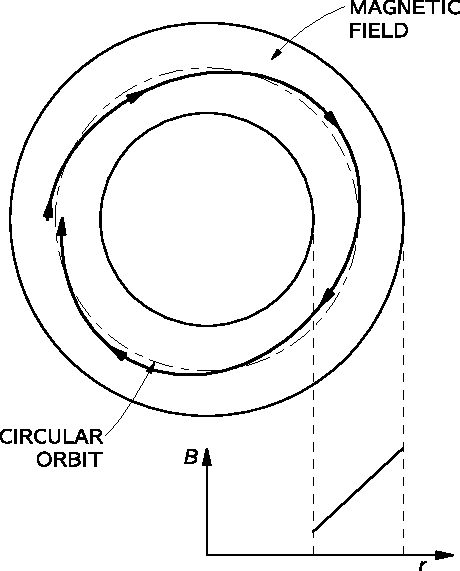
\includegraphics[width=0.7\linewidth]{fyz_fig633.pdf}
      \caption{
               (\cite[s.~707]{Feynman02})}
      \label{fyz_fig633}
    \end{figure}

    \begin{figure}[ht!] %\ref{fyz_fig634}
      \centering
      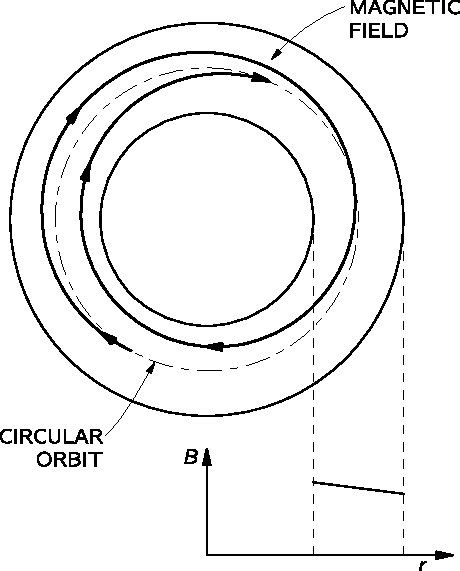
\includegraphics[width=0.7\linewidth]{fyz_fig634.pdf}
      \caption{
               (\cite[s.~707]{Feynman02})}
      \label{fyz_fig634}
    \end{figure}

    \begin{figure}[ht!] %\ref{fyz_fig635}
      \centering
      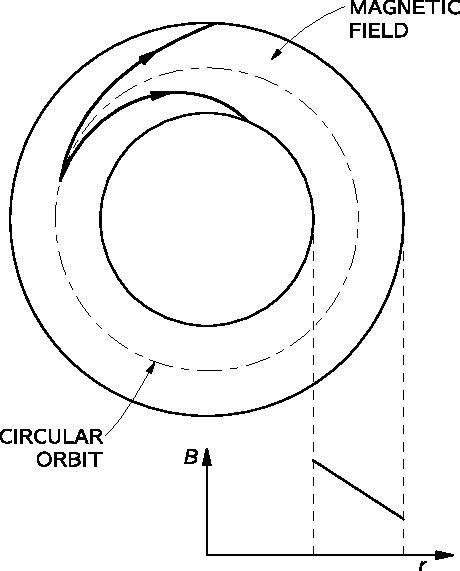
\includegraphics[width=0.7\linewidth]{fyz_fig635.pdf}
      \caption{
               (\cite[s.~707]{Feynman02})}
      \label{fyz_fig635}
    \end{figure}

    \begin{figure}[ht!] %\ref{fyz_fig636}
      \centering
      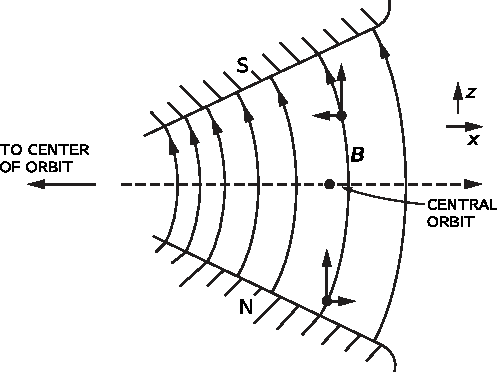
\includegraphics[width=0.7\linewidth]{fyz_fig636.pdf}
      \caption{
               (\cite[s.~707]{Feynman02})}
      \label{fyz_fig636}
    \end{figure}

    \begin{figure}[ht!] %\ref{fyz_fig637}
      \centering
      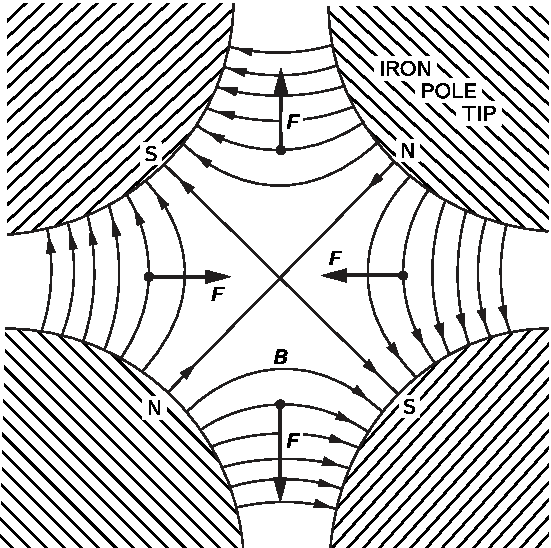
\includegraphics[width=0.7\linewidth]{fyz_fig637.pdf}
      \caption{
               (\cite[s.~707]{Feynman02})}
      \label{fyz_fig637}
    \end{figure}

    \begin{figure}[ht!] %\ref{fyz_fig638}
      \centering
      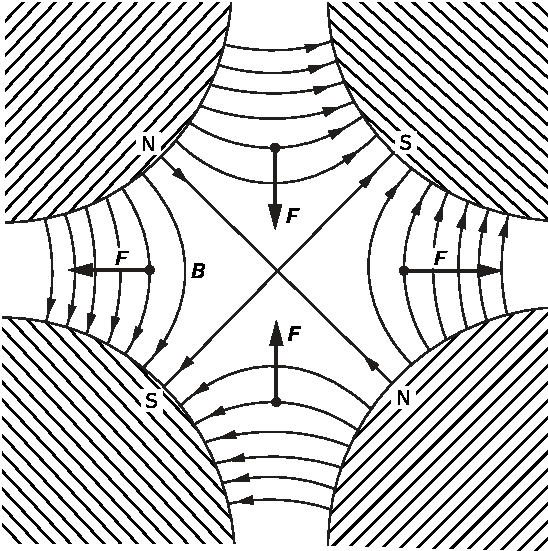
\includegraphics[width=0.7\linewidth]{fyz_fig638.pdf}
      \caption{
               (\cite[s.~707]{Feynman02})}
      \label{fyz_fig638}
    \end{figure}

    \begin{figure}[ht!] %\ref{fyz_fig639}
      \centering
      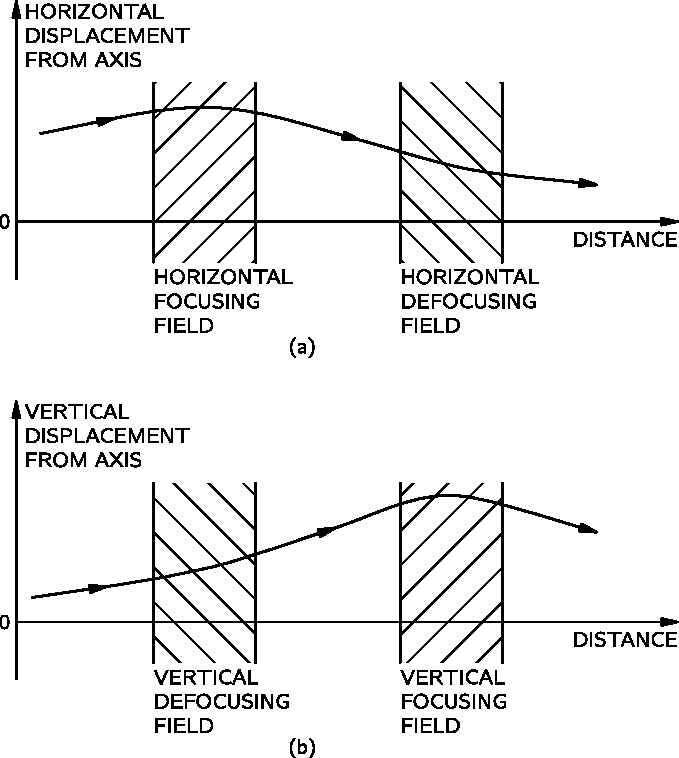
\includegraphics[width=0.7\linewidth]{fyz_fig639.pdf}
      \caption{
               (\cite[s.~707]{Feynman02})}
      \label{fyz_fig639}
    \end{figure}

    \begin{figure}[ht!] %\ref{fyz_fig640}
      \centering
      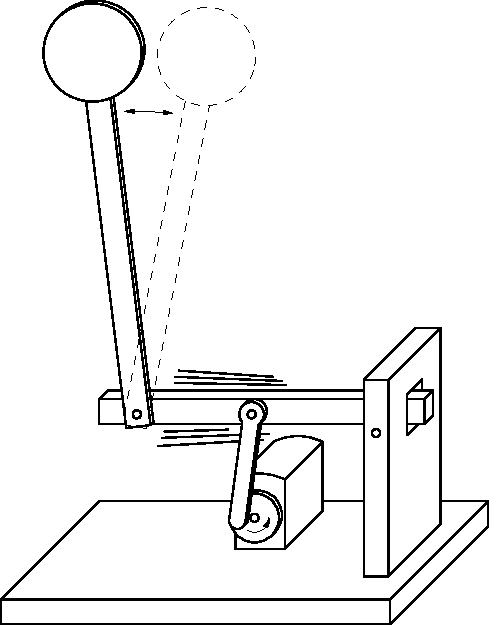
\includegraphics[width=0.7\linewidth]{fyz_fig640.pdf}
      \caption{
               (\cite[s.~707]{Feynman02})}
      \label{fyz_fig640}
    \end{figure}

    \begin{figure}[ht!] %\ref{fyz_fig641}
      \centering
      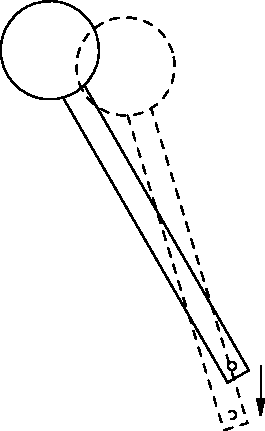
\includegraphics[width=0.7\linewidth]{fyz_fig641.pdf}
      \caption{
               (\cite[s.~707]{Feynman02})}
      \label{fyz_fig641}
    \end{figure}

    \begin{figure}[ht!] %\ref{fyz_fig642}
      \centering
      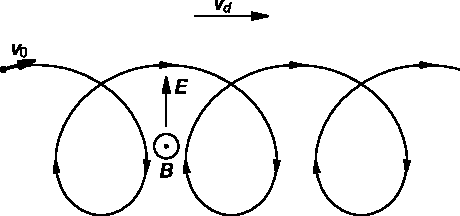
\includegraphics[width=0.7\linewidth]{fyz_fig642.pdf}
      \caption{
               (\cite[s.~707]{Feynman02})}
      \label{fyz_fig642}
    \end{figure}



} %tikzset
%---------------------------------------------------------------------------------------------------
\printbibliography[title={Seznam literatury},heading=subbibliography]
\addcontentsline{toc}{section}{Seznam literatury}